\documentclass{article}
\usepackage{amsmath}
\usepackage{amssymb}
\usepackage{amsbsy}
\usepackage{bbm}
\usepackage{url}
\usepackage{color}
\usepackage{graphicx}
\usepackage{epstopdf}
\usepackage{fancyhdr}
\usepackage{enumerate}
\usepackage{tikz}
\usepackage[ruled,vlined]{algorithm2e}
\usepackage[colorlinks=true,urlcolor=blue]{hyperref}
\usepackage[utf8]{inputenc}

\title{Homework 2}
\author{Sara Bizjak, sb6054@student.uni-lj.si}

\newcommand{\Solution}[1]{{\medskip \color{black} \bf $\bigstar$~\sf \textbf{Solution}~$\bigstar$ \sf #1 } \bigskip}

\begin{document}

\maketitle

%%%%%%%%%%%%%%%%%%%%%%%%%%%%%%%%%%%%%%%%%%%%%%%%%%%%%%%%%%%%%%%%%%%%%%%%%%%%%%%%%%%%%%%%%%%%%%%%%%%%%%%%%%%%
%%%%%%%%%%%%%%%%%%%%%%%%%%%%%%%%%%%%%%%%%%%%%%%%%%%%%%%%%%%%%%%%%%%%%%%%%%%%%%%%%%%%%%%%%%%%%%%%%%%%%%%%%%%%

\section{GCN}
\subsection*{Question 1.1}
\Solution{

\noindent
  The two given graphs are isomorphic. The isomorphism between two graphs can be defined as a function $\Phi: V(G_1) \to V(G_2)$ that maps together the following pairs of nodes.
  \begin{itemize}
    \begin{minipage}{0.5\textwidth}
    \item $1 \to A$
    \item $2 \to D$
    \item $3 \to H$
    \item $4 \to E$
    \end{minipage}
    \begin{minipage}{0.5\textwidth}
    \item $5 \to B$
    \item $6 \to C$
    \item $7 \to G$
    \item $8 \to F$
    \end{minipage}
  \end{itemize}
  or more clearly, 1-to-1 correspondence between nodes and edges is presented on the figure below.

  \begin{figure}[ht!]
    \centering
    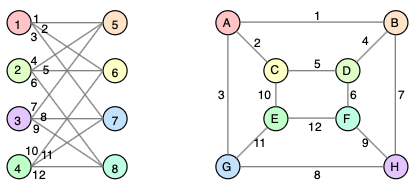
\includegraphics[width=90mm]{Slike/1_1.png}
    \caption{Visualization of isomorphism between two given graphs. Correspondence between nodes is denoted with the same coloring and between edges with the same assigned number.}
  \end{figure}
  \noindent
  More mathematically, $\Phi$ is a homomorphism and bijection, and $\Phi^{-1}$ is homomorphism, so it follows that $\Phi$ is isomorphism.
}

%%%%%%%%%%%%%%%%%%%%%%%%%%%%%%%%%%%%%%%%%%%%%%%%%%%%%%%%%%%%%%%%%%%%%%%%%%%%%%%%%%%%%%%%%%%%%%%%%%%%%%%%%%%%

\subsection*{Question 1.2}
\Solution{

  \noindent
  \begin{figure}[ht!]
    \centering
    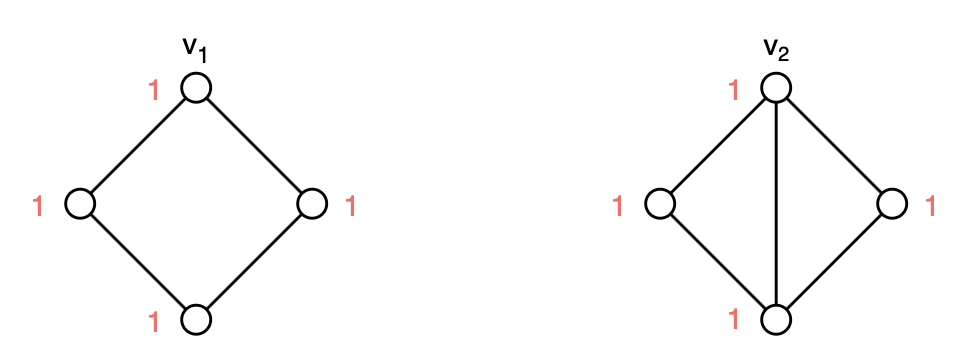
\includegraphics[width=90mm]{Slike/1_2.png}
    \caption{Example of two graphs that satisfy the conditions in the instructions.}
  \end{figure}

\noindent
Let assume the graphs $G_1$ and $G_2$ as in the figure above, with assigned initial features $1$ for every node, following 
that $h_{v_1}^{(0)} = h_{v_2}^{(0)}$ holds. 
Then we have, using each of the three aggregations, 
\begin{itemize} 
  \item Mean aggregation: $h_{v_1}^{(1)} = \frac{1 + 1}{2} = 1$ and $h_{v_2}^{(1)} = \frac{1 + 1 + 1}{3} = 1$.
  \item Max aggregation: $h_{v_1}^{(1)} = \max(1, 1) = 1$ and $h_{v_2}^{(1)} = \max(1, 1, 1) = 1$.
  \item Sum aggregation: $h_{v_1}^{(1)} = 1 + 1 = 2$ and $h_{v_2}^{(1)} = 1 + 1 + 1 = 3$.
\end{itemize}
so the updated features $h_{v_1}^{(1)}$ and $h_{v_2}^{(1)}$ are equal if we use mean and max aggregation, but different if we use sum aggregation.
}

%%%%%%%%%%%%%%%%%%%%%%%%%%%%%%%%%%%%%%%%%%%%%%%%%%%%%%%%%%%%%%%%%%%%%%%%%%%%%%%%%%%%%%%%%%%%%%%%%%%%%%%%%%%%

\subsection*{Question 1.3}
\Solution{

  \noindent
  Let $G_1$ and $G_2$ be non-isomorphic graphs and their node embeddings are updated over $K$ iterations 
  with the same \texttt{aggregate$(.)$} and \texttt{combine$(.)$} functions.
  \\
  We suppose that \texttt{readout}$\left( \left{ h_v^{(K)}, \forall v \in V_1 \right}\right) \neq$ \texttt{readout}$\left( \left{ h_v^{(K)}, \forall v \in V_2 \right}\right)$
  and then prove that WL test also decides the graphs are not-isomorphic.
  \\
  We will prove this using the contradiction, thus assume that WL after $K$ iterations cannot decide if $G_1$ and $G_2$ are not-isomorphic.
  %So by the WL algorithm it follows that
  %\begin{align}
  %\{l_v^{(i)}, \ \forall v \in V_1 \} = \{l_v^{(i)}, \ \forall v \in V_2 \}  \ \ \ \forall i = 0, 1, \ldots, K
  %\end{align}
  \\
  Graphs $G_1$ and $G_2$  have the same node labels labels $\{ l_v^{i}\}$ as well as the same set of neighborhoods 
  $\left\{ \left( l_v^{(i)}, \left\{ l_u^{(i)}: u \in N(v) \right\}\right)\right\}$
  for iterations $i$ and $i + 1$ for any $i = 0, 1, \ldots, K-1$.
  If that would not be true, the WL test would have obtained different collections of node labels for graph $G_1$ and $G_2$ at iteration $i + 1$, since different multisets always get different new labels.
  \\
  We now show that for same graphs $G_1 = G_2$, if WL test labels nodes as $l_v^{(i)} = l_u^{(i)}$, we have the same GNN embeddings for nodes $v$ and $u$ at the $i$-th iteration, so $h_v^{(i)} = h_u^{(i)}$ holds for ant iteration $i$.
  \\
  This is obviously true for $i = 0$, since WL and GNN starts with the same node features. From there, we apply induction.
  Suppose this hold for iteration $j$, so in $(j + 1)$-th iteration we have $l_v^{(j + 1)} = l_u^{(j + 1)}$ for every pair of nodes $u$ and $v$, meaning that
  \begin{align*}
    \left\{ \left( l_v^{(j)}, \left\{ l_w^{(j)}: w \in N(v) \right\}\right)\right\} = \left\{ \left( l_u^{(j)}, \left\{ l_w^{(j)}: w \in N(u) \right\}\right)\right\}
  \end{align*}
  and also 
  \begin{align*}
    \left\{ \left( h_v^{(j)}, \left\{ h_w^{(j)}: w \in N(v) \right\}\right)\right\} = \left\{ \left( h_u^{(j)}, \left\{ h_w^{(j)}: w \in N(u) \right\}\right)\right\}
  \end{align*}
  The same input in GNN produces the same output, since the same \texttt{agregate(.)} and \texttt{combine(.)} functions are used. 
  Therefore, the condition $h_v^{(j + 1)} = h_u^{(j + 1)}$ holds, meaning that we can find a mapping $\phi$, such that $\phi(l_v^{(i)}) = h_v^{(i)}$ for any $v$ from a graph $G_1$ or $G_2$.
  It follows that all $\{h_v^{(i + 1)}\}$ are the same, thus the readout functions for both graphs $G_1$ and $G_2$ are also the same.
  By this assumption, we have reach a contradiction, meaning that WL test says $G_1$ and $G_2$ are not-isomorphic.


}


%%%%%%%%%%%%%%%%%%%%%%%%%%%%%%%%%%%%%%%%%%%%%%%%%%%%%%%%%%%%%%%%%%%%%%%%%%%%%%%%%%%%%%%%%%%%%%%%%%%%%%%%%%%%
%%%%%%%%%%%%%%%%%%%%%%%%%%%%%%%%%%%%%%%%%%%%%%%%%%%%%%%%%%%%%%%%%%%%%%%%%%%%%%%%%%%%%%%%%%%%%%%%%%%%%%%%%%%%


\section{Node Embeddings with TransE}

\subsection*{Question 2.1}
\Solution{

  \noindent
Assume we have the graph presented in the figure below. 
\begin{figure}[ht!]
  \centering
  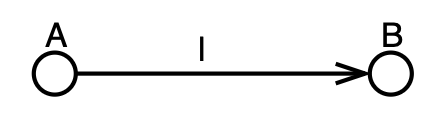
\includegraphics[width=40mm]{Slike/2_1.png}
  \caption{Graph example.}
\end{figure}

\noindent
Let's set the embedding of nodes $A$ and $B$ to be $[1, 0]^T$ and of $l$ to be $[0, 0]^T$, thus the condition $[1, 0]^T + [0, 0]^T = [1, 0]^T$ is ensured as proposed.
Then is follows
\begin{align*}
  \mathcal{L}_{simple} = d \left( \begin{bmatrix} 1 \\ 0 \end{bmatrix} + \begin{bmatrix} 0 \\ 0 \end{bmatrix}, \begin{bmatrix} 1 \\ 0 \end{bmatrix} \right) = d \left( \begin{bmatrix} 1 \\ 0 \end{bmatrix}, \begin{bmatrix} 1 \\ 0 \end{bmatrix} \right) = 0
\end{align*}
thus the $\mathcal{L}_{simple}$ is minimized to 0. The embedding of the graph is, however, useless, since we cannot distinguish the nodes.
}

%%%%%%%%%%%%%%%%%%%%%%%%%%%%%%%%%%%%%%%%%%%%%%%%%%%%%%%%%%%%%%%%%%%%%%%%%%%%%%%%%%%%%%%%%%%%%%%%%%%%%%%%%%%%

\subsection*{Question 2.2}
\Solution{

  \noindent
  Assume we have the same graph as before, with the same, useless embeddings.
  Then, following the equation
  \begin{align*}
    \mathcal{L}_{no margin} = \sum_{(h, l, t) \in S} \sum_{(h', l, t') \in S'_{(h, l, t)}} \left[ d(h+ l, t) - d(h' + l, t') \right]_{+}
  \end{align*}
  it is abvious that $\mathcal{L}_{no margin}  = 0$, since the first part in the bracket, $d(h+ l, t) = 0$ for every $(h, l, t) \in S$.
  The second part is, again, the function $d(.,.)$, the Euclidean distance, which in general is greater or equal 0.
  Therefore, every member of the sum $\left[ d(h+ l, t) - d(h' + l, t') \right]_{+}$ is equal to 0 (since $[.]_{+}$ is the positive part function, defined as $\max(0,.)$).
  Thus, the sum of zeros is equal to 0 and condition $ \mathcal{L}_{no margin} = 0$ holds.
}

%%%%%%%%%%%%%%%%%%%%%%%%%%%%%%%%%%%%%%%%%%%%%%%%%%%%%%%%%%%%%%%%%%%%%%%%%%%%%%%%%%%%%%%%%%%%%%%%%%%%%%%%%%%%

\subsection*{Question 2.3}
\Solution{

  \noindent
  To normalize every entity embedding is importat if we want to prevent the training process to trivially minimize the $\mathcal{L}$.
  To be precise, for triples $(h, l, t) \in S$ the algorithm will choose the embeddings that are close together, 
  i.~e.~the norm of embeddings of $h$ and $t$ would be about the same size, and embeddings for triples $(h', l, t') \in S'$ would choose to be far apart.
  Not normalizing the embeddings would mean that they could get bigger with every iteration, so the $d(h' + l, t')$ would outgrow the first part of the equation ($\gamma + d(h+ l, t)$)
  and the loss $\mathcal{L}$ would, by the defition of $[.]_+$, become 0.
}




%%%%%%%%%%%%%%%%%%%%%%%%%%%%%%%%%%%%%%%%%%%%%%%%%%%%%%%%%%%%%%%%%%%%%%%%%%%%%%%%%%%%%%%%%%%%%%%%%%%%%%%%%%%%

\subsection*{Question 2.4}
\Solution{

  \noindent
  Recall from the lectures: TransE cannot model 1-to-N and symmetric relations. 
  \\
  Let's explain the example with 1-to-N relation on a simple graph, presented on a figure below.
  \begin{figure}[ht!]
    \centering
    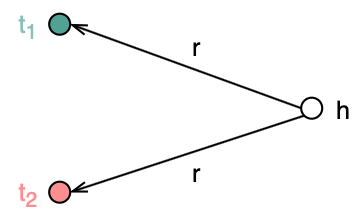
\includegraphics[width=50mm]{Slike/2_4.png}
    \caption{Graph example.}
  \end{figure}
  Since the nodes $t_1$ and $t_2$ are different, i.~e.~colored in different colors, we want them to have different embeddings, so we can distinguish them.
  According to the drawing of a graph, 
  \begin{align}
    t_1 = h + r
    \\
    t_2 = h + r
    \\
    t_1 \neq t_2
  \end{align}
  From (1) and (2) it follows that $t_1$ and $t_2$ will be mapped to the same vector, although they are different entities. 
  By that, we came to contradiction, since we set the embeddings to be different (condition (3)).
  Therefore, for any choice of different embeddings for $t_1$ and $t_2$, we cannot find such embedding of relation vector $r$ to satisfy the conditions (1), (2) and (3) at the same time,
  so the graph has no perfect embedding.

}

%%%%%%%%%%%%%%%%%%%%%%%%%%%%%%%%%%%%%%%%%%%%%%%%%%%%%%%%%%%%%%%%%%%%%%%%%%%%%%%%%%%%%%%%%%%%%%%%%%%%%%%%%%%%
%%%%%%%%%%%%%%%%%%%%%%%%%%%%%%%%%%%%%%%%%%%%%%%%%%%%%%%%%%%%%%%%%%%%%%%%%%%%%%%%%%%%%%%%%%%%%%%%%%%%%%%%%%%%

\section{Expressive Power of Knowledge Graph Embeddings}

\subsection*{Question 3.1}
\Solution{

  \noindent
  \textbf{Symmetry.} TransE cannot model symmetric relations.
  \\
  \textit{Proof.} Assume that it can. Then, the embedding equations $h + l = t$ and $t + l = h$ hold, thus the only solution to solve this is that $l = 0$ and $h = t$.
  However, we cannot have $h = t$, since $h$ and $t$ are different entities and should, therefore, have different embeddings.
  \\
  \\
  \textbf{Inverse.} TransE can model inverse relations. 
  \\
  \textit{Proof.} Let's have the equations $h + l_1 = t$ (1) and $t + l_2 = h$ (2). The solution, i.~e.~the inverse, would simply be $l_2 = - l_1$ (cond.).
  More intuitively, if we imagine a graph with two nodes of the embeddings $h$ and $t$, $l_1$ and $l_2$ would be the directed connections between two nodes in both ways, so we can just say that one is the opposite or inverse direction of the other (or vector in the opposite direction).
  \begin{figure}[ht!]
    \centering
    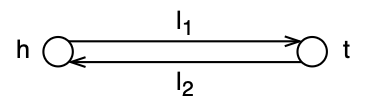
\includegraphics[width=50mm]{Slike/3_a_2.png}
    \caption{Graph example for inverse explanation.}
  \end{figure}

  \noindent
  Formally,
  \begin{align*}
    t + l_2 &= h \ \ \ \ \ \ \ \ \ \text{write (2) + use (cond.)}
    \\
    t - l_1 &= h 
    \\
    t &= h + l_1 \ \ \ \text{get (1)}
  \end{align*}
  which is the case.
  \\
  \\
  \textbf{Composition.} TransE can model composition.
  \\
  \textit{Proof.} Let's have the equations $h + l_1 = t$ (1), $t + l_2 = f$ (2) and $h + l_3 = f$ (3). If we solve this, we get $l_3 = l_1 + l_2$ (cond.).
  More intuitively, we can imagine this as a graph representation drawn in a triangle, following $l_3 = l_1 + l_2$ can be imagined as a vector sum.
  \begin{figure}[ht!]
    \centering
    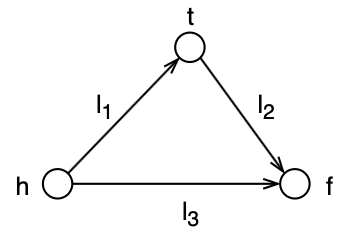
\includegraphics[width=50mm]{Slike/3_a_3.png}
    \caption{Graph example for composition explanation.}
  \end{figure}

  \noindent
  Formally,
  \begin{align*}
    h + l_3 &= f \ \ \ \text{write (3) + use (cond.)}
    \\
    h + l_1 + l_2 &= f \ \ \ \ \text{use (1)}
    \\
    h + l_2 &= f \ \ \ \text{get (2)}
  \end{align*}
  which is the case.
  }

%%%%%%%%%%%%%%%%%%%%%%%%%%%%%%%%%%%%%%%%%%%%%%%%%%%%%%%%%%%%%%%%%%%%%%%%%%%%%%%%%%%%%%%%%%%%%%%%%%%%%%%%%%%%

\subsection*{Question 3.2}
\Solution{

  \noindent
  \textbf{Symmetry.} RotateE can model symmetry.
  \\
  \textit{Proof.} Let assume the symmetry, so the equations $h \circ l = t$ and $t \circ l = h$ hold. Let set $l$ such that $l \circ l = 1$ is true.
  Then we have $ t \circ l = (h \circ l) \circ l = h \circ (l \circ l) = h$ so the condition holds and symmetry is proved.
  \\
  \\
  \textbf{Inverse.} RotateE can model inverse.
  \\
  \textit{Proof.} Let assume the inverse, so the equations $h \circ l_1 = t$ (1) and $t \circ l_2 = h$ (2) hold. The solution, i.~e.~the inverse, 
  would simply be $l_2 = l_1^{-1}$ (cond.), so that $l_1 \circ l_2 = 1$. Formally,
  \begin{align*}
    t \circ l_2 &= h \ \ \ \ \ \ \ \ \text{write (2) + use (cond.)}
    \\
    t \circ l_1^{-1} &= h 
    \\
    t &= h \circ l_1 \ \ \ \text{get (1)}
  \end{align*}
  which is the case.
  \\
  \\
  \textbf{Composition.} RotateE can model composition.
  \\
  \textit{Proof.} Let assume the composition, so the equations $h \circ l_1 = t$ (1), $t \circ l_2 = f$ (2) and $h \circ l_3 = f$ (3) hold. 
  The solution would simply be $l_3 = l_1 \circ l_2$ (cond.). Formally,
  \begin{align*}
    h \circ l_3 &= f \ \ \ \text{write (3) + use (cond.)}
    \\
    h \circ l_1 \circ l_2 &= f \ \ \ \text{use (1)}
    \\
    t \circ l_2 &= f \ \ \ \text{get (2)}
  \end{align*}
  which is the case.
  }

%%%%%%%%%%%%%%%%%%%%%%%%%%%%%%%%%%%%%%%%%%%%%%%%%%%%%%%%%%%%%%%%%%%%%%%%%%%%%%%%%%%%%%%%%%%%%%%%%%%%%%%%%%%%

\subsection*{Question 3.3}
\Solution{

  \noindent
  RotateE cannot model 1-to-N realtions.
  \\
  Let assume we have the same graph as before (with TransE in Question 2.4.) and the proof goes exactly the same as for TransE.
  \begin{figure}[ht!]
    \centering
    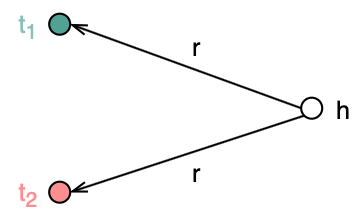
\includegraphics[width=50mm]{Slike/2_4.png}
    \caption{Graph example.}
  \end{figure}
Since the nodes $t_1$ and $t_2$ are different, i.~e.~colored in different colors, we want them to have different embeddings, so we can distinguish them.
According to the drawing of a graph, 
\begin{align*}
  h \circ r = t_1
  \\
  h \circ r = t_2
\end{align*}
following that $t_1 = t_2$ which is in contradiction with $t_1$ and $t_2$ having different embeddings.
}

%%%%%%%%%%%%%%%%%%%%%%%%%%%%%%%%%%%%%%%%%%%%%%%%%%%%%%%%%%%%%%%%%%%%%%%%%%%%%%%%%%%%%%%%%%%%%%%%%%%%%%%%%%%%
%%%%%%%%%%%%%%%%%%%%%%%%%%%%%%%%%%%%%%%%%%%%%%%%%%%%%%%%%%%%%%%%%%%%%%%%%%%%%%%%%%%%%%%%%%%%%%%%%%%%%%%%%%%%

\section{Honor Code}
(X) I have read and understood Stanford Honor Code before I submitted my work.
\\ $**$ Collaboration: Maruša Oražem (63200439), Vid Stropnik (63200434).$**$
\\
\\
\begin{figure}[ht!]
  \centering
  
\includegraphics[width=120mm]{Slike/cover.png}
\end{figure}






\end{document}
